%%%%%%%%%%%%%%%%%%%%%%%%%%%%%%%%%%%%%%%%%%%%%%%%%%%%%%%%%%%%%%%%%
%%% %
%%% % weiiszablon.tex
%%% % The Faculty of Electrical and Computer Engineering
%%% % Rzeszow University Of Technology diploma thesis Template
%%% % Szablon pracy dyplomowej Wydziału Elektrotechniki 
%%% % i Informatyki PRz
%%% % June, 2015
%%%%%%%%%%%%%%%%%%%%%%%%%%%%%%%%%%%%%%%%%%%%%%%%%%%%%%%%%%%%%%%%%

\documentclass[12pt,twoside]{article}

\usepackage{weiiszablon}

\author{Damian Bielecki}

% np. EF-123456, EN-654321, ...
\studentID{EF-163461}
\title{Śledzenie obiektów przez robota mobilnego z wykorzystaniem głębokiej sieci neuronowej}
\titleEN{Temat pracy po angielsku}


%%% wybierz rodzaj pracy wpisując jeden z poniższych numerów: ...
% 1 = inżynierska	% BSc
% 2 = magisterska	% MSc
% 3 = doktorska		% PhD
%%% na miejsce zera w linijce poniżej
\newcommand{\rodzajPracyNo}{1}


%%% promotor
\supervisor{dr.hab.inż Krzysztof Wiktorowicz prof. PRz}
%% przykład: dr hab. inż. Józef Nowak, prof. PRz

%%% promotor ze stopniami naukowymi po angielsku
\supervisorEN{(academic degree) Imię i nazwisko opiekuna}

\abstract{Treść streszczenia po polsku}
\abstractEN{Treść streszczenia po angielsku}

\begin{document}

% strona tytułowa
\maketitle

\blankpage

% spis treści
\tableofcontents

\clearpage
\blankpage

\section{Wprowadzenie}

Obserwując rynek możemy zauważyć ciągły wzrost liczby urządzeń będących coraz bardziej inteligentnych
i odpornych na ciągle zmieniające się otoczenie.

Celem projektu inżynierskiego jest zbudowanie robota śledzącego wskazany obiekt, który jest wykryty przez zamontowaną na nim kamerę.
Robot będzie sterowany przez komputer przetwarzający obraz przy pomocy odpowiednio wytrenowanej
głębokiej sieci neuronowej. Zadaniem sieci będzie rozpoznanie i zlokalizowanie wyznaczonego obiektu, 
a następnie przekazanie jego pozycji algorytmu sterującego. Dalsza część programu
wyśle odpowiednio spreparowane komendy do robota, aby ten ustawił karetkę z kamerą na obiektem.

Głównym powodem realizacji takiego tematu jest chęć poznania działania i trenowania głębokich sieci 
neuronowych rozpoznających obiekty na obrazach.

\textbf{Omówienie rozdziałów}

Mając na uwadze zakres pracy i cel projektu, jej treść podzielono na szereg rozdziałów. 
Rozdział pierwszy ogólnie omawia typy i zasadę działania sieci neuronowych. 
Rozdział drugi skupia się na przeglądzie literatury, a w szczególności na opisie istniejących rozwiązań
wykorzystujących rozpoznawanie obiektów przy pomocy głębokiej sieci neuronowej.
Rozdział trzeci szczegółowo omawia proces budowy wykorzystywanego dalej robota.
Rozdział czwarty opisuje proces pozyskania danych i trenowania sieci rozpoznającej obiekty.
Rozdział piąty omawia utworzony program wykorzystujący wytrenowaną sieć neuronową, cały proces sterowania i 
sposób połączenia wszystkich systemów w działający projekt.
Ostatni rozdział przedstawia testy finalnej wersji programu oraz ich krótki opis. 


\section{Omówienie działania głębokich sieci neuronowych}
\subsection{Wprowadzenie do sieci neuronowych}

Podstawowymi elementami strukturalnymi, z których buduje się sztuczne sieci 
neuronowe są neurony. Każdy neuron posiada wejścia, na które podawane są 
sygnały mnożone przez odpowiednie wagi, sumowane, a następnie po przejściu przez 
funkcje aktywacji kierowane na wyjście neuronu. 


\begin{figure}[H]
	\centering
	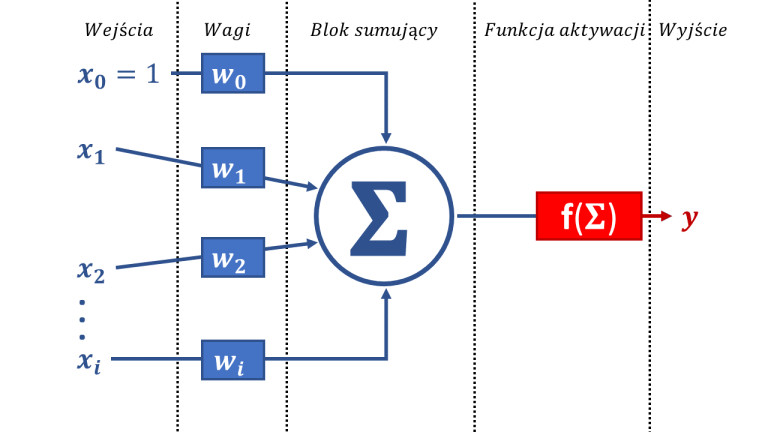
\includegraphics[width=12cm]{pages/teoria/zdjecia/sztucznyNeuron.jpg}
	\caption{Schemat pojedynczego neuronu \cite{sztucznyNeuron}}
	\label{rys:ogolnyRozwiazania}
\end{figure}


Wyjście powyższego neuronu możemy opisać wzorem:

\begin{equation}
	y = f( \sum_{i = 0}^{N}w_i x_i) = f(W^T x)
	\label{eq:rownanieNeuronu}
\end{equation}
Gdzie: $x=[1, x_1, x_2, ..., x_N]$ - to wektor sygnałów wejściowych (1 na początku wektora odpowiada
za przesunięcie), $W = [w_0, w_1, w_2, ..., w_N]$ - jest wektorem wag ($w_0$ to wartość progowa aktywacji),
$f(x)$ to wybrana funkcja aktywacji

\textbf{Najczęściej stosowane funkcje aktywacji:}

\begin{equation}
	f(x) = \frac{1}{1 + e^-x\beta} 
	\label{eq:signum}
\end{equation}

\begin{equation}
	f(x) = \frac{e^x - e^-x}{e^x + e^-x}
	\label{eq:tangensHiperboliczny}
\end{equation}

\begin{equation}
	f(x) = \begin{cases}
		1 & gdy x \> 0 \\
		0 & gdy x <  0
	\end{cases}
	\label{eq:skokuJednostkowego}
\end{equation}


\textbf{Wielowarstwowe sieci neuronowe}

W praktycznym zastosowaniu sieć zbudowana z jednej warstwy neuronów nie pozwoli nam na osiągnięcie satysfakcjonujących wyników.
Możemy określić dwa typy sieci pod względem ilości warstw: 
\begin{itemize}
	\item Uczenie maszynowe - zazwyczaj są zbudowane z trzech warstw (ukryta-ukryta-wyjściowa) 
	\item Głębokie uczenie - posiada dużo więcej warstw neuronów, w skomplikowanych sieciach nawet kilkaset
\end{itemize}

Relacje pomiędzy nimi przedstawia poniższy schemat
\begin{figure}[H]
	\centering
	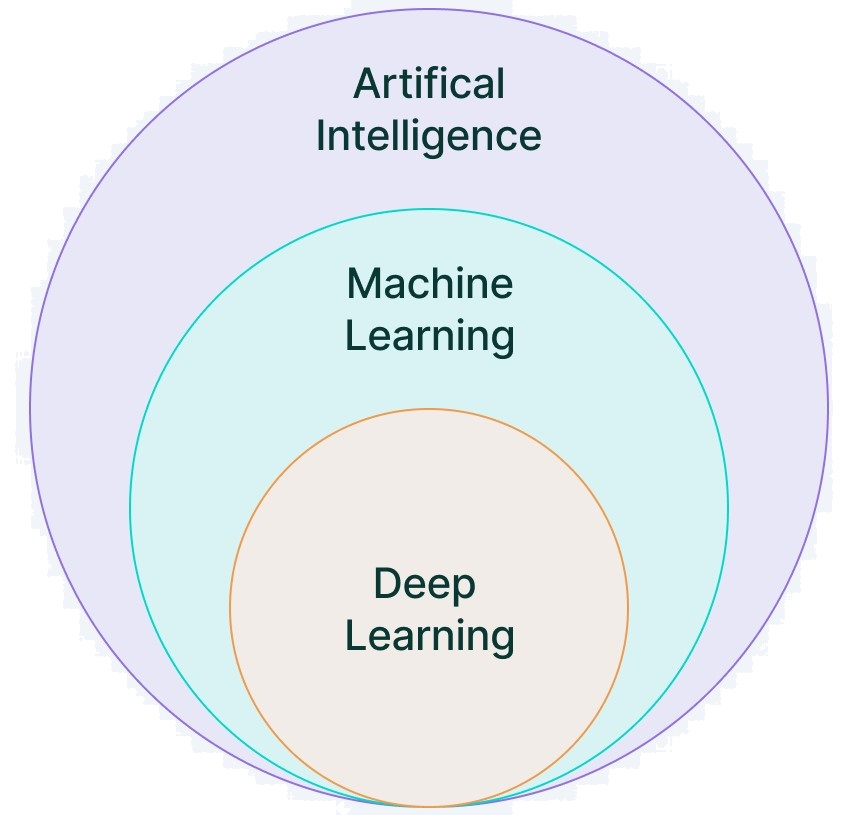
\includegraphics[width=10cm]{pages/teoria/zdjecia/schematAI.jpg}
	\caption{Relacja pomiędzy typami sieci neuronowych \cite{schematAISite}}
	\label{rys:schematAI}
\end{figure}


\subsection{Głębokie sieci neuronowe}


\subsection{Algorytmy detekcji obiektów na zdjęciach}





\clearpage

\addcontentsline{toc}{section}{Literatura}
\begin{thebibliography}{4}
    \bibitem{sztucznyNeuron} https://batmaja.com/sztuczny-neuron/ Dostęp 07.01.2023
    \bibitem{schematAISite} https://www.v7labs.com/blog/machine-learning-guide Dostęp 07.01.2023
% \bibitem{str} http://weii.portal.prz.edu.pl/pl/materialy-do-pobrania. Dostęp 5.01.2015.
\end{thebibliography}

\clearpage

% \makesummary

\end{document} 
